\documentclass{article}
\usepackage{graphicx}
\usepackage{graphicx}
\usepackage{subfig}

\title{Facial Emotion Recognizer on VGG16}
\author{Fazzari, Fabro, Spaziani, Locchi }
\date{July 2023}

\begin{document}

\maketitle
\tableofcontents

\newpage
\section{Introduction}

For our project we decided to create a model that recognizes,given a human face, the emotions felt.
Our chosen architecture and datasete were respectively the VGG16, and FER-2013.

\begin{figure}[htbp]
    \centering
    
    \subfloat[Real time facial emotion recognition]
    {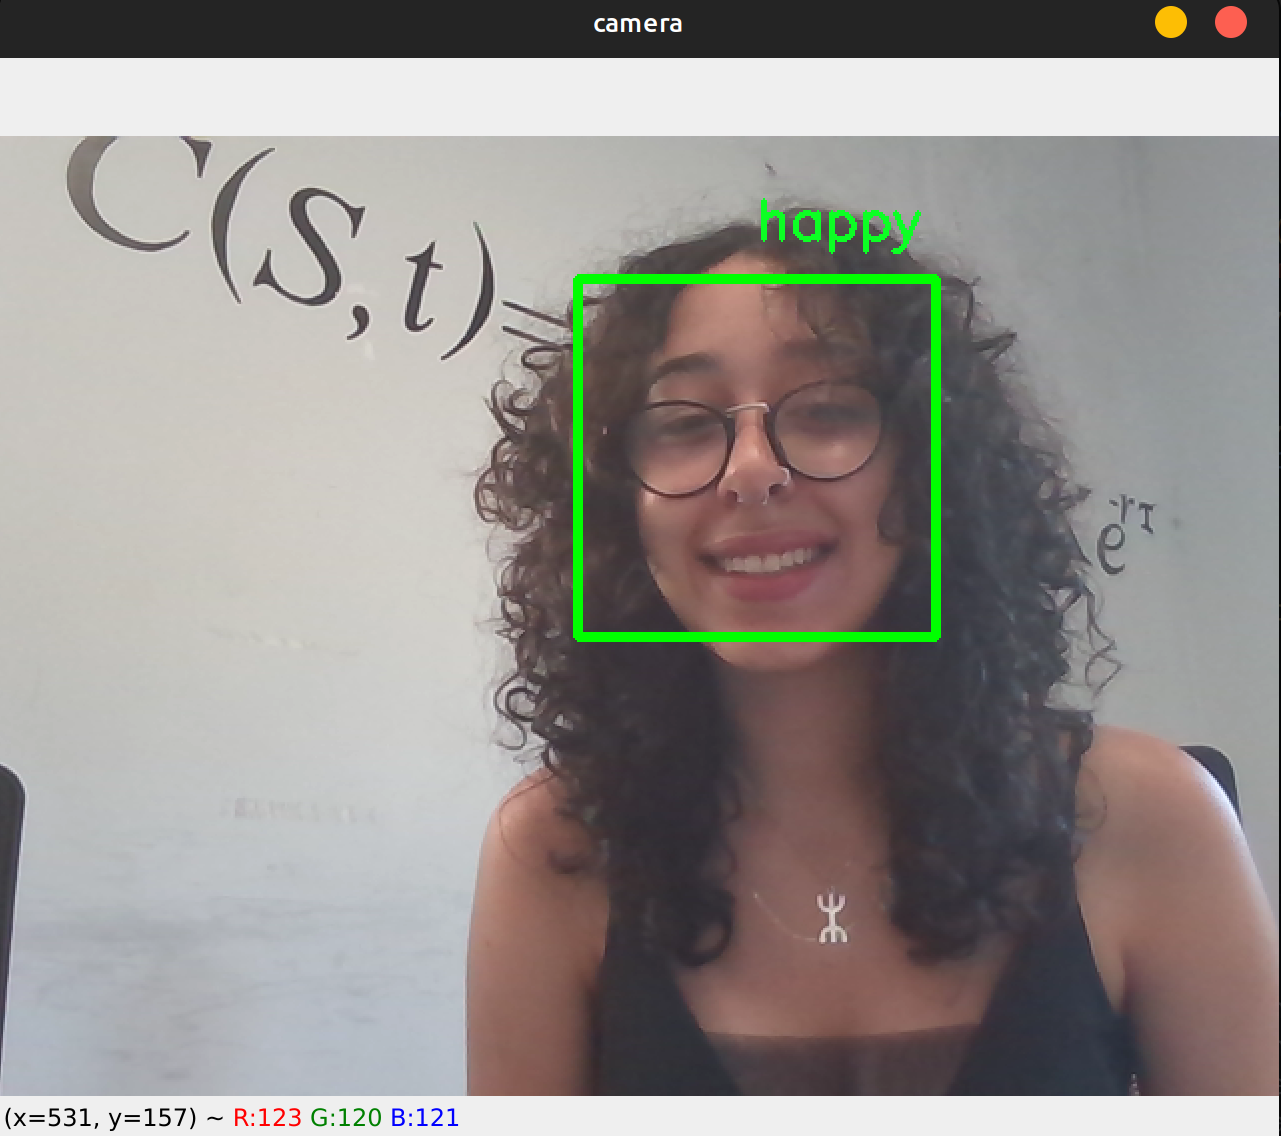
\includegraphics[width=0.4\textwidth]{imgs/introduction/introduction_img2.png}}
    \hfill
    \subfloat[Some test results] {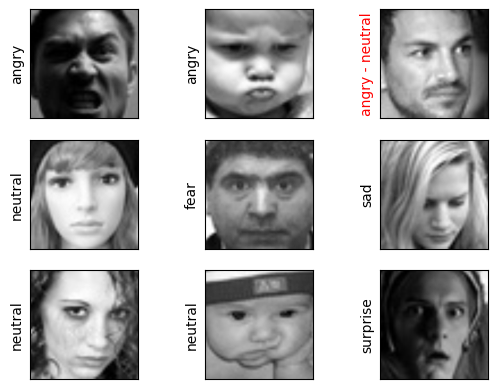
\includegraphics[width=0.5\textwidth]{imgs/introduction/introduction_img1.png}}
    \label{fig:introduction_img}
\end{figure}

\newpage
\section{The Model}
The chosen model was the VGG16, in our opinion the best choice,since it gives great results while keeping the architecture simple.

The architecture is built as it follows:

Once the preprocessed image is input to the model, it goes through a series of computations in the forward pass. The forward pass involves passing the image through the different layers of the model. Each layer performs specific operations on the input, such as convolutions, activations, pooling.
As the image progresses through the layers of the model, it undergoes a process of feature extraction. Lower layers in the model capture low-level features like edges, corners, and textures, while deeper layers capture higher-level features and semantic information. This hierarchical feature extraction allows the model to learn representations that are progressively more complex and meaningful.
The final layers of the model consist of three fully connected layers. These layers take the extracted features from the previous layers and map them to the desired output classes.
The weight init is xavier\_uniform\_

\begin{figure}[htbp]

\centering
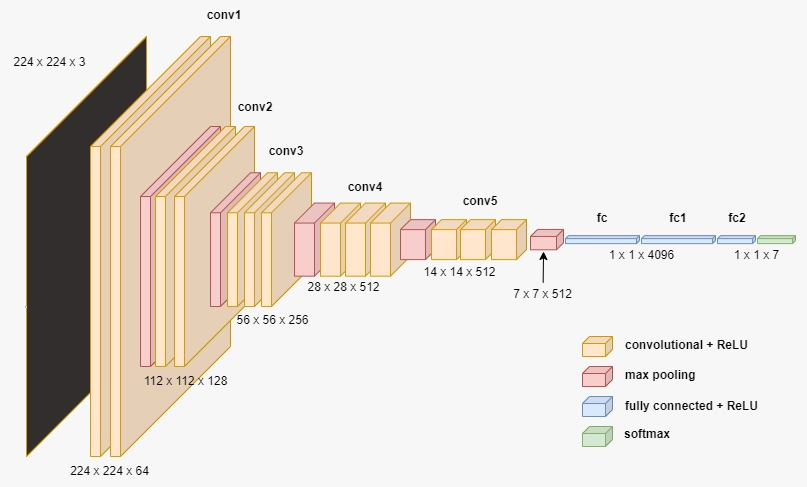
\includegraphics[width=\textwidth]{imgs/model_arch.jpeg}

\caption{Model Architecture}
\label{fig:dataset_img}

\end{figure}

\newpage
\section{The Dataset}
the chosen dataset is the FER20213, it presents a meager number of 48x48, black and white images (35.000), representing faces seen from the front, and from slightly different angles. We split the dataset in "train", "validation" and "test". The validation sub-set was created by extracting 10\% of the train sub-set images.

\begin{figure}[htbp]

\centering
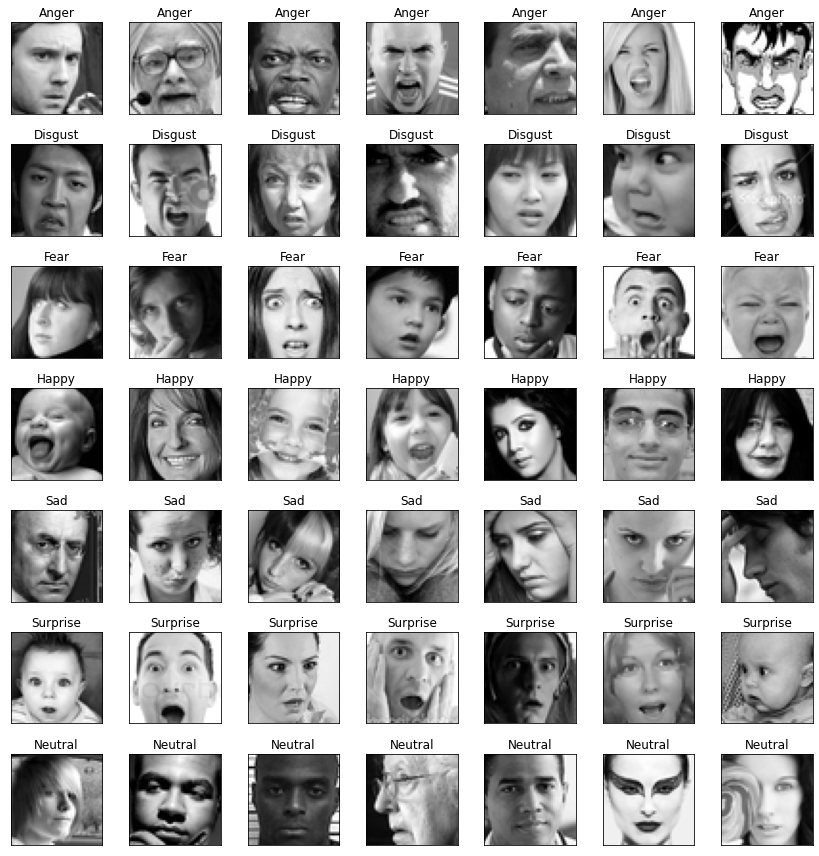
\includegraphics[width=0.45\textwidth]{imgs/dataset/dataset_img2.png}

\caption{Real time facial emotion recognition}
\label{fig:dataset_img}

\end{figure}

Since the VGG16 expects 224x244, 3-channeled images, after running some tests,we decided to adapt the dataset to our architecture,enhancing the prediction of some specific classes.


\newpage
\section{Tuning}
To train our model we tried different parameters and optimizer, lastly we chose the ones that performed better,comparing them with the values of similar projects.
\begin{figure}[htbp]

\centering
\includegraphics[width=0.4\textwidth]{imgs/tuning/AdamW batch_size:64 lr: 0.0001.png}

\caption{Best AdamW performance}
\label{fig:tuning_img}

\end{figure}

We tested with other optimizers like SGD and Adam, these are the results:
\begin{figure}[htbp]
\centering
\subfloat[Best Adam performance]{
\includegraphics[width=0.35\textwidth]{imgs/tuning/Adam batch_size:64 lr: 0.0001.png}}
\hspace{1cm}
\subfloat[Best SGD performance]
{\includegraphics[width=0.35\textwidth]{imgs/tuning/SGD batch_size:64 lr: 0.0001.png}}
\label{fig:tuning_img}
\end{figure}

Lastly,our choice,even tho it gave similar results compared to Adam, was AdamW, since it's better management of the weight decay.

We present our model with the so-tuned parameters optimizer and loss function:
\begin{itemize}
  \item Ottimizzatore: AdamW
  \item Funzione di Loss: CrossEntropyLoss
  \item Epoch: 50
  \item Early Stopping: 20
  \item Parametri finali:
  \begin{itemize}
    \item Learning rate (lr): 0.0001
    \item Weight decay: $5 \times 10^{-4}$
  \end{itemize}
\end{itemize}



\section{Final Result}
The results after training our model over the dataset are the following:
\begin{table}[htbp]
\centering
\caption{Performance Metrics}
\label{tab:performance_metrics}
\resizebox{0.55\textwidth}{!}{
\begin{tabular}{ccccccc}
\hline
Class & Precision & Recall & F1-Score & Support \\
\hline
Surprise & 0.7740 & 0.7750 & 0.7745 & 831 \\
Fear & 0.5171 & 0.3545 & 0.4206 & 1024 \\
Angry & 0.4663 & 0.6712 & 0.5503 & 958 \\
Neutral & 0.5737 & 0.6123 & 0.5924 & 1233 \\
Sad & 0.5275 & 0.4531 & 0.4875 & 1247 \\
Disgust & 0.2793 & 0.4505 & 0.3448 & 111 \\
Happy & 0.8664 & 0.8298 & 0.8477 & 1774 \\
\hline
Accuracy & & & 0.6258 & 7178 \\
Macro Avg & 0.5721 & 0.5923 & 0.5740 & 7178 \\
Weighted Avg & 0.6342 & 0.6258 & 0.6244 & 7178 \\
\hline
\end{tabular}
}
\end{table}

A big flaw of our model is its low accuracy, even after a long testing period,we couldn't improve it. 
Although,we can still use it for some simple yet fancy functionality
\begin{figure}[htbp]
\centering
\subfloat[Test Confusion Matrix]{
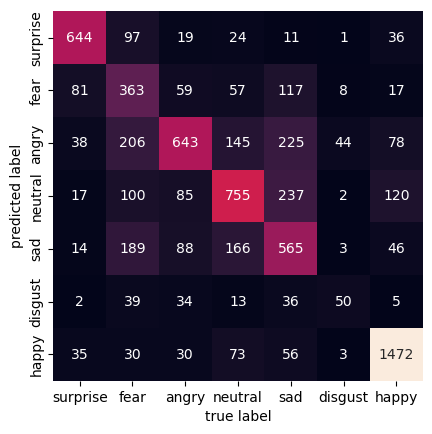
\includegraphics[width=0.35\textwidth]{imgs/final_result/confusion_matrix.png}}
\label{fig:final_result_img}
\end{figure}


\section{Real Time Emotion Detection}
To make better use of our model, we decided to implement a simple paralleled feature to demonstrate our work in practice.
To do this, we took advantage of the capabilities of OpenCV.
Our script consists of taking frames from OpenCV's VideoCapture and pass them to a function of ours that takes advantage of the HaarCascades algorithm that recognizes faces and allows us to return a list of coordinates, which indicates the rectangle of the recognized portion of the face, and the image of the face cropped. So we can pass the image to the model,with the coordinates shown in real time and the recognized portion of the face, via an interrupt the user can request the recognition of the emotion and eventually the result is shown on the screen above the recognized face. In addition, this system also works with multiple faces conteporately due to the very face recognition algorithm used.
\begin{figure}[htbp]
\centering
\subfloat[CiZ and Andrea]{
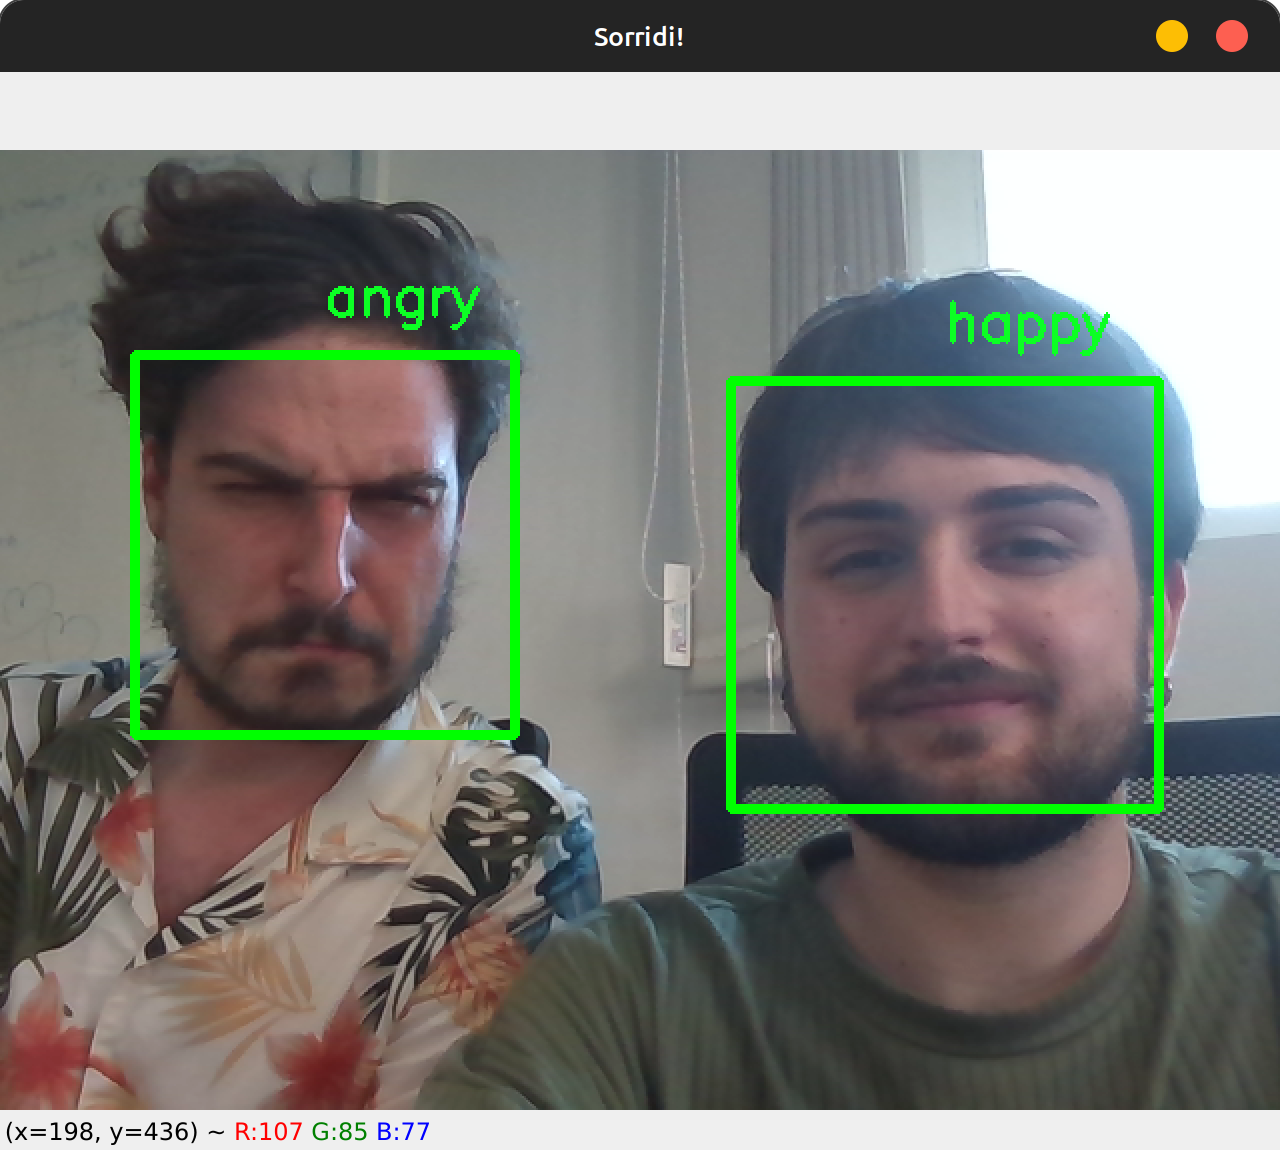
\includegraphics[width=0.45\textwidth]{imgs/side_quest/rt_detect1.png}}
\label{fig:sidequest_img}
\end{figure}


\end{document}